\chapter*{Light Curves}


\subsection*{Switching Catalogs}\\[5mm]
 "After reviewing the Libralato, Bedin, Nardiello $\&$ Piotto (2015) paper (url listed below), Chelsea realized that one possible improvement we could make would be to update our catalog. We had been using a catalog named \textbf{photref.cat} which contained less than 10,000 sources. I took the variable sources listed in the Asiago Input Catalog, which contained more than 75,935 sources. Some of these sources were actually slightly outside the field of view of K2, so this was actually reduce to 66,486 sources in the end. The file \texttt{m35n2158\_kepmag.out} is in the directory \texttt{/home/msoares/chelseasrc/ims/CATALOG}. Also in this subdirectory is the former catalog \texttt{photref.cat}. \\
The catalog contains the following information:
ID (integer number to identify source)   RA (J2000)   DEC (J2000)   Kepmag (mag)
Kepler magnitudes range from 7.5 to 31.2. 
The  catalog originally contained the sources in B-mag, V-mag, R-mag, J-mag, H-mag, K-mag, and instrument N-mag. More info on this catalog is given here. I had to convert these values to the Kepler magnitudes. To do this, I followed the logic given in the EPIC manual on page 10: \url{https://archive.stsci.edu/k2/epic.pdf}"\\

\textit{add a step to the routine that generates the cmrawphot file to search for double entries and assign a new name to the second source (e.g., I might call it "HAT-264-0576773.2")}

Libralato et al. 2015 \url{http://arxiv.org/pdf/1510.09180v2.pdf}

\subsection*{Addressing double catalog entries}
"There is a bug(/"feature") in the UCAC4 catalog in which certain sources that were resolved as multiple objects in some of the catalogs contributing to UCAC4, but only a single source in the 2MASS catalog, are given separate entries for each component in UCAC4. Each source has the same 2mass ID and is thus assigned the same HAT ID by our ucac4read code. The result is that I end up with a handful of sources having the same name in the cmrawphot file, leading to double entries for that id in the output photometry and double entries for each cadence in the light curve." \\ 
ID this problem for the effected sources: (ie)
\begin{enumerate}
\item HAT-264-0576773
\item HAT-264-0011034
\item HAT-264-0003844
\item \sout{HAT-264-0345492} -- recently deleted because the file was null
\item \sout{HAT-264-0113691}
\item \sout{HAT-264-0001303}
\end{enumerate}

\textit{What do we do with these files?}\\
"Joel says that it is not obvious what the best way to deal with this is. 
Obviously we need to fix something in the higher level catalog query step, but they haven't decided what that fix would be. 
We have previously discussed assigning new HATIDs to the fainter stars in each pair, but this requires fudging the 2MASS IDs in the catalog and we would still like to keep track of their original degenerate matches to 2MASS.  
Joel's suggestion would be to manually split the .rlc light curves into two for each of the objects above -- I can do this either by \textbf{relative position} or \textbf{reference brightness}."

Melinda addressed this issue by writing a script that separated the .rlc files. Her post-TFA .rlc files have been separated. The script is located at \texttt{msoares/Dropbox/K20/Notebooks/170504\_SeparatingFiles.ipynb}.



\subsection*{Investigating Reduced Light Curves to Find Candidates}
To perform the Box-fitting Least Squares (BLS) and the Lomb-Scargle algorithms (Scargle, 1982), we will use two methods: Joel Hartman's Vartools script and Waqas Bhatti's interactive, visually intuitive, and Astrobase code (written in Python).

\begin{enumerate}
    \item find and classify interesting candidates interactively using Python pickles and Bhatti's Astrobase Checkplotserver webapp, This sets and saves variability tags, object type tags, best periods and epochs, and comments for each object using a browser-based UI.
   
    \item The information entered can then be exported as CSV or JSON, see \url{https://github.com/waqasbhatti/astrobase/blob/master/notebooks/lightcurves-and-checkplots.ipynb}, melinda has pickle file \texttt{TFA\_LC\_PKL}.
    
    \item make a \texttt{.json} file using the command \texttt{checkplotlist pkl}
    
    \item view them with checkplotserver by typing \texttt{checkplotserver}
\end{enumerate}

\begin{center}
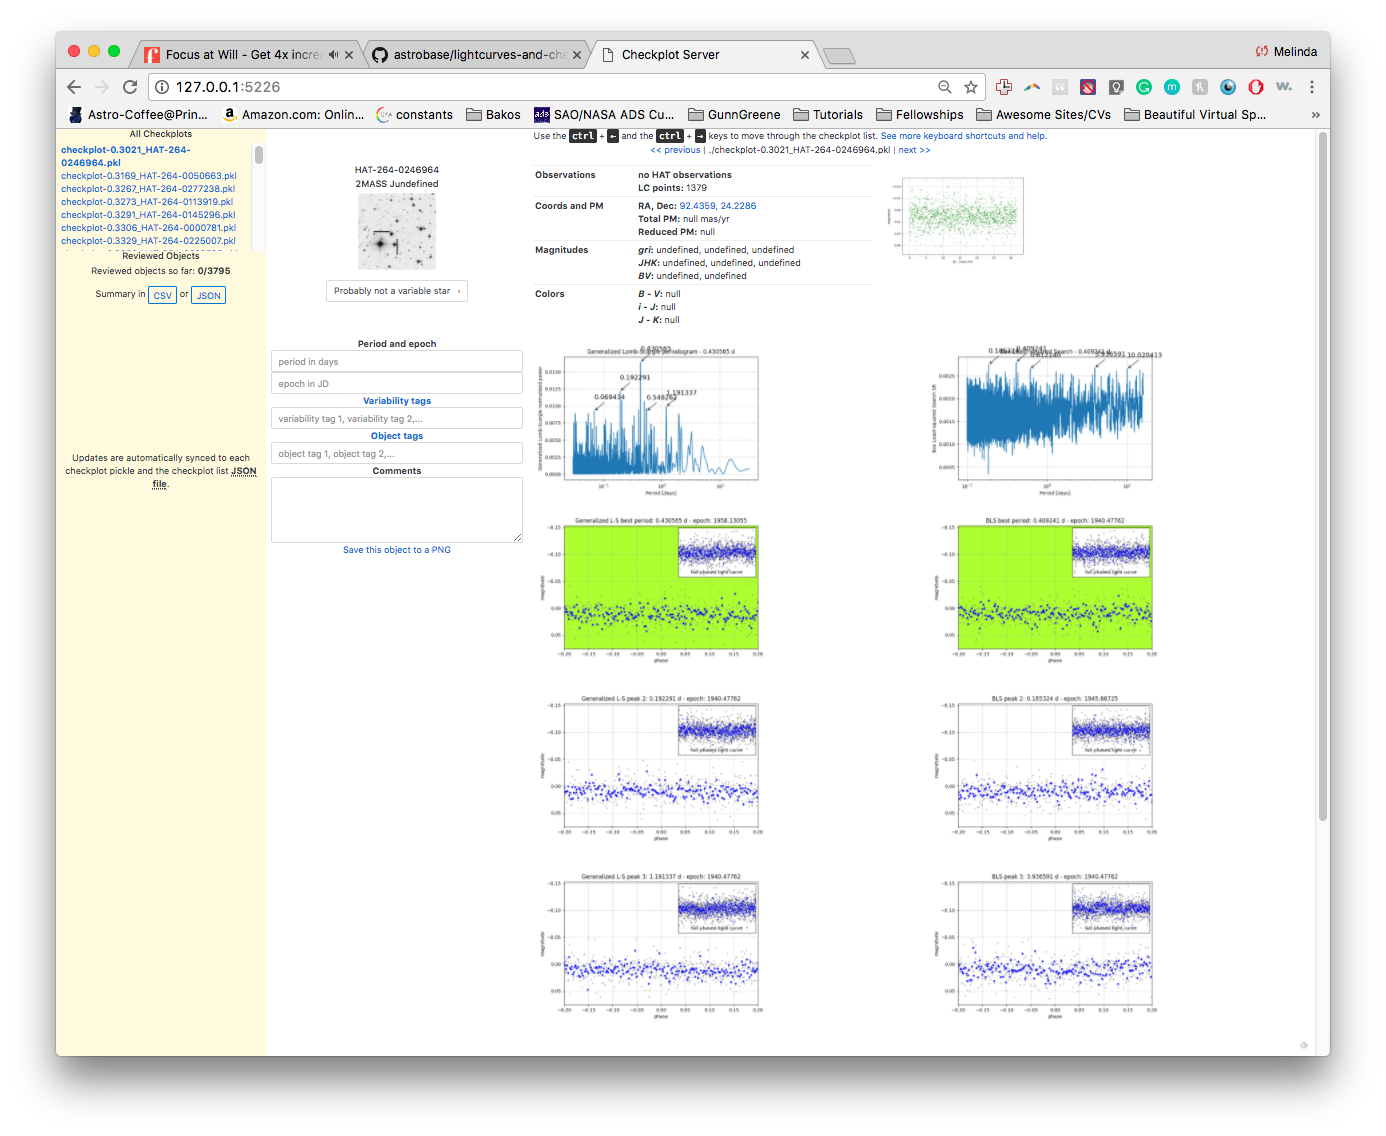
\includegraphics[width=0.7\textwidth]{melinda/checkplotserver.png}\\
\end{center}
When you save objects as a .png file, they will save within the same \texttt{TFA\_LC\_PKL} subdirectory, so you'll need to move them to an appropriate folder. 


\subsection*{Vartools Output Lightcurves}
The Vartools output files, on the other hand, are located on the phs11 machine at the subdirectory \texttt{/home/msoares/chelseasrc/ims/BLS/BLS_1}

Here there are two types of files, the phase curve, which contains phase information and the magnitude of the model, ends in *.rlc.tfalc.bls.phcurve, while those ending in *.rlc.tfalc.bls.model contain the model. The plot shown in Figure~\ref{finalfile} only relies on the contents of the *.rlc.tfalc.bls.phcurve files. 

\s*{Running Parallelized Scripts for Faster Analysis}
\section*{Using ipyparallel}
I got another technically helpful email from Waqas explaining how to use ipyparallel to run BLS and LS algorithms using his Astrobase software. You cannot just use multiprocessing.Pool here, as it will error out due to the spawning of daemonic processes. 
I can still run stuff in parallel, but only if I switch
to ipyparallel as the driver instead of multiprocessing.Pool. This
mostly follows the advice in the notebook:
\url{https://github.com/waqasbhatti/astrobase/blob/master/notebooks/parallel-ipython.ipynb}

Essentially, I run ipyparallel workers on the same machine instead of across a cluster. How do I do this?

With your virtualenv activated:
\begin{minted}{bash}
    (venv)$ pip install ipyparallel
\end{minted}
That will install the driver and workers.

Then to start a cluster on phs11 with 4 workers (as laid out before):
\begin{minted}{bash}
    (venv)$ ipcluster start -n 4 &
\end{minted}

Then I simply follow the notebook from ``set up the cluster view" onwards.
The function I map across the whole cluster is my
worker function that I set up for use with multiprocessing.Pool. The function call is very similar:

\begin{minted}{bash}
    results = dview.map_sync(do_lc_stuff, lclist)
\end{minted}

 Melinda has a script to run the tfa step:    \texttt{/home/msoares/chelseasrc/ims/Astrobase/Parallel_MakeTFA_LC_PNG_Vartools.py}

\section*{Submit with nohup}
Pipes break and they break often, as a result, you really need to use nohup with all file submissions. Here is an example of how to run your parallelized script using nohup to prevent these issues.

\begin{minted}{bash}
    (venv)$ nohup ipcluster -n 4 >> error-log.txt &

    (venv)$ nohup python /path/to/your/script.py >> error-log.txt &
\end{minted}


\Huge{NONE of this has been edited}
\subsection*{Collecting the Light Curves}
Light curve collection is performed by calling the program \textbf{grcollect}. \\
See Chelsea's bash script \textbf{lc\_gen.sh}. 
The script takes a input list, which we have named \textbf{iphot.ls}. This input list contains frame names without an extension or pathway.
I can open the input list iphot.ls as an example. 
I then tell the script where the lightcurve goes by changing the value of LC.
The script reads in all the iphot (photometry) files at one time, and match the measurement for the same star from different frames, and output light curve files (.rlc).
Lightcurves are being generated and saved to the pathway \textbf{/nfs/phs11/ar0/S/PROJ/msoares/201509\_K20\_ISM\_OpenClusters/IMSUB/LC/}.
You run the script with the command \textbf{./lc\_gen.sh}, however I have renamed this to \textbf{melinda\_lc\_gen.sh}\\
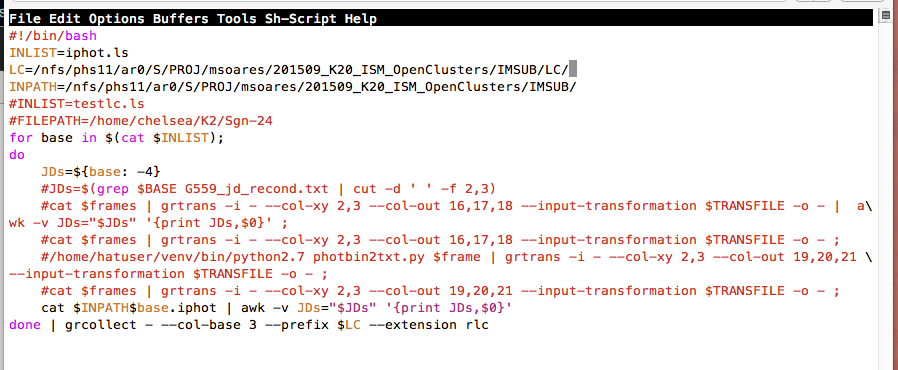
\includegraphics[width=0.9\textwidth]{lcgen.png}\\
\\ \\ 

\section*{Comparing Light Curves}
The next step is to compare my newly generated lightcurves to those published by other sources (Nardiello et al. 2014). 
I should start with things brighter than \textbf{13th V-mag} and with \textbf{variation amplitude $>$ 1\%}.\\ \textcolor{red}{\textit{How do I check variation amplitude? Is this just as easy as it sounds?}}\\
This would give a solid first impression for the quality of our light curve. 
I will then gradually go down on mag and precision during the fine tuning process. 

I need the HAT ID number in order to compare light curves, To get this, I need the RA and DEC (in degrees) of the star, which is conveniently given in the catalog table of the Nardiello paper.
The command to run to determine the HAT ID for a given RA and DEC is: \\ 
\textbf{2massread -r ra -d dec -s 0.005 --cat /S/CAT/2MASS/2MASS\_JH\_AP/data/}.\\
This command is querying a star within 0.0005 degrees of the given RA and DEC. This really is the limit on how finely resolved we should make the query program. If multiple stars are within this field, I will need to look at the J and H magnitudes of the star to distinguish it from neighbors. 
I wrote the script \textbf{FindHatID.py}, which finds a HATID for a requested RA and DEC value. 
Output looks like the image below: \\
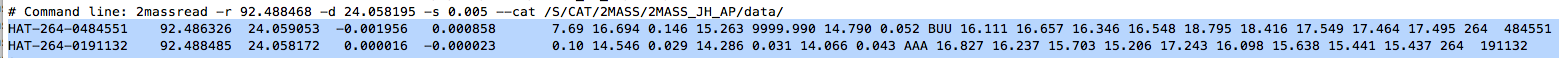
\includegraphics[width=\textwidth]{HATID.png}\\
The 7th column is the J-2MASS magnitude and the 9th column is the H-2MASS magnitude, which are both given in the catalog table in Nardiello et al. 2014. In this instance, we want HATID number \textbf{HAT-264-0191132}. This ID number is the title of the \textbf{.rlc} file of interest.\\
The larger Nardiello et al. catalog is given here:\\
\url{http://vizier.cfa.harvard.edu/viz-bin/VizieR-3?-source=J/MNRAS/447/3536/variable}\\ \\ 
I will be comparing the light curves of 10 selected objects. These stellar objects, their coordinates, their magnitudes, and the corresponding HAT ID numbers are given in the table below.


\begin{table}[]
\centering
\label{my-label}
\begin{tabular}{|c|c|c|c|c|c|c|c|}
\hline
\textbf{Star} & \textbf{RA} & \textbf{DEC} & \textbf{Type} & \textbf{$V_{\rm 2MASS}$} & \textbf{$J_{\rm 2MASS}$} & \textbf{$H_{\rm 2MASS}$} & \textbf{HAT ID} \\ \hline
%\textbf{Star} & \textbf{RA} & \textbf{DEC (+)} & \textbf{Type} & \textbf{V\_2MASS} & \textbf{J\_2MASS} & \textbf{H\_2MASS} & \textbf{HAT ID} \\ \hline
514           & 92.113065   & 24.328803        & EB            & 10.072            & 9.919             & 9.889             & HAT-264-0002367 \\ \hline
509           & 92.314359   & 24.258219        & Rot           & 10.175            & 9.918             & 9.957             & HAT-264-0002364 \\ \hline
506           & 92.439300   & 24.214583        & Rot           & 10.390            & 10.082            & 10.099            & HAT-264-0002883 \\ \hline
516           & 92.248379   & 24.366616        & Rot           & 10.685            & 10.256            & 10.260            & HAT-264-0264752 \\ \hline
512           & 92.199523   & 24.295566        & Rot           & 10.709            & 10.318            & 10.317            & HAT-264-0003539 \\ \hline
497           & 92.225659   & 24.369275        & Rot           & 10.874            & 10.493            & 10.460            & HAT-264-0004259 \\ \hline
517           & 92.45543    & 24.401628        & EB            & 12.569            & 11.527            & 11.460            & HAT-264-0016758 \\ \hline
508           & 92.128748   & 24.253384       & EB   		   & 12.744            & 11.648             & 11.399             & HAT-264-0016779 \\ \hline
513           & 92.409717   & 24.298180        & EB            & 12.924             & 11.262              & 10.961             & HAT-264-0012457 \\ \hline
515           & 91.971587   & 24.353585       & EB             & 13.132 & 12.150	           & 11.969              & HAT-264-0023455 \\ \hline

\end{tabular}
\caption{Comparison Selection for Light Curves  -Taken from Nardiello et al. 2014}
\label{Nard}
\end{table}

\section*{Generate the Light Curve}
Example walk-through:\\
I now have a file of interest, which in this case is file \textbf{HAT-264-0191132.rlc}. This is just a text file with lots of ``null'' values therein. 
I have a cadence column (column 1), and lots of magnitude columns. 
Next, \textit{for now},  I go on to download all \textbf{.rlc} plots, so I can use the interactive iPython notebook format to generate scripts. 
I'm currently using the notebook \textbf{2015\_1015\_PlotLightCurve.ipynb} to generate light curves for now. 
For now, I am ignoring optimization of the aperture selection for now. This will be the final step after I have finely tuned all other parameters.
\textit{Behold}, I can now plot magnitude vs. time, where $t \rm = 2456727.0219333335+cadence \times \frac{0.5}{24}- 2456000$ 
I am generating light curves in an interactive format using plotly. You can see my interactive plotly gallery at:\\
\url{https://plot.ly/~msoares/}.

\section*{First Light Curve Batch Results: \hl{\textbf{b}/2, \textbf{i}/3, and \textbf{d}=3/3}}
I generated light curves for the ten Nardiello sources listed in Table \ref{Nard}. These ten were selected because they were bright in J-magnitude. I preferentially selected eclipsing binaries when possible and ignored long period variables, where variability would be unlikely to be seen given our observation window. Unfortunately, this initial attempt was not successful. The oscillations shown in the light curves were caused by the variations due to drift and were not real photometric variations. 
The immediate next step was to \textcolor{red}{\textit{create a few sets of light curves varying the image subtraction parameters, and using a photometry master frame with each of the reference frames "ficonv"ed first.}}\\
Chelsea recommends the following parameter variation format:
\begin{itemize}
\item -k part of the ficonv command... changing the number after b/, i/ and d=;\\
where b/ controls the order of the polynomials fit to the background, i/ controls the order of polynomials we fit to the flux term of the kernel, and d=x/y, x is the size of the half size of the discrete kernel, y is the polynomial order. For all the numbers, Chelsea wouldn't go higher than 4.
She suspects x should be small, right now d=3/3, maybe I should try x=1 and 2 first. 
\end{itemize}
As recommended by Joel, I computed the standard deviation of each light curve and generated a scatter plot of average magnitude vs standard deviation for each aperture size. Joel claims that these plots are often informative diagnostics. 
This was generated using the code \textbf{StndVMag.py}. A snapshot of the script is shown below with the first containing HATSOUTH points overplotted for reference. 
\begin{center}
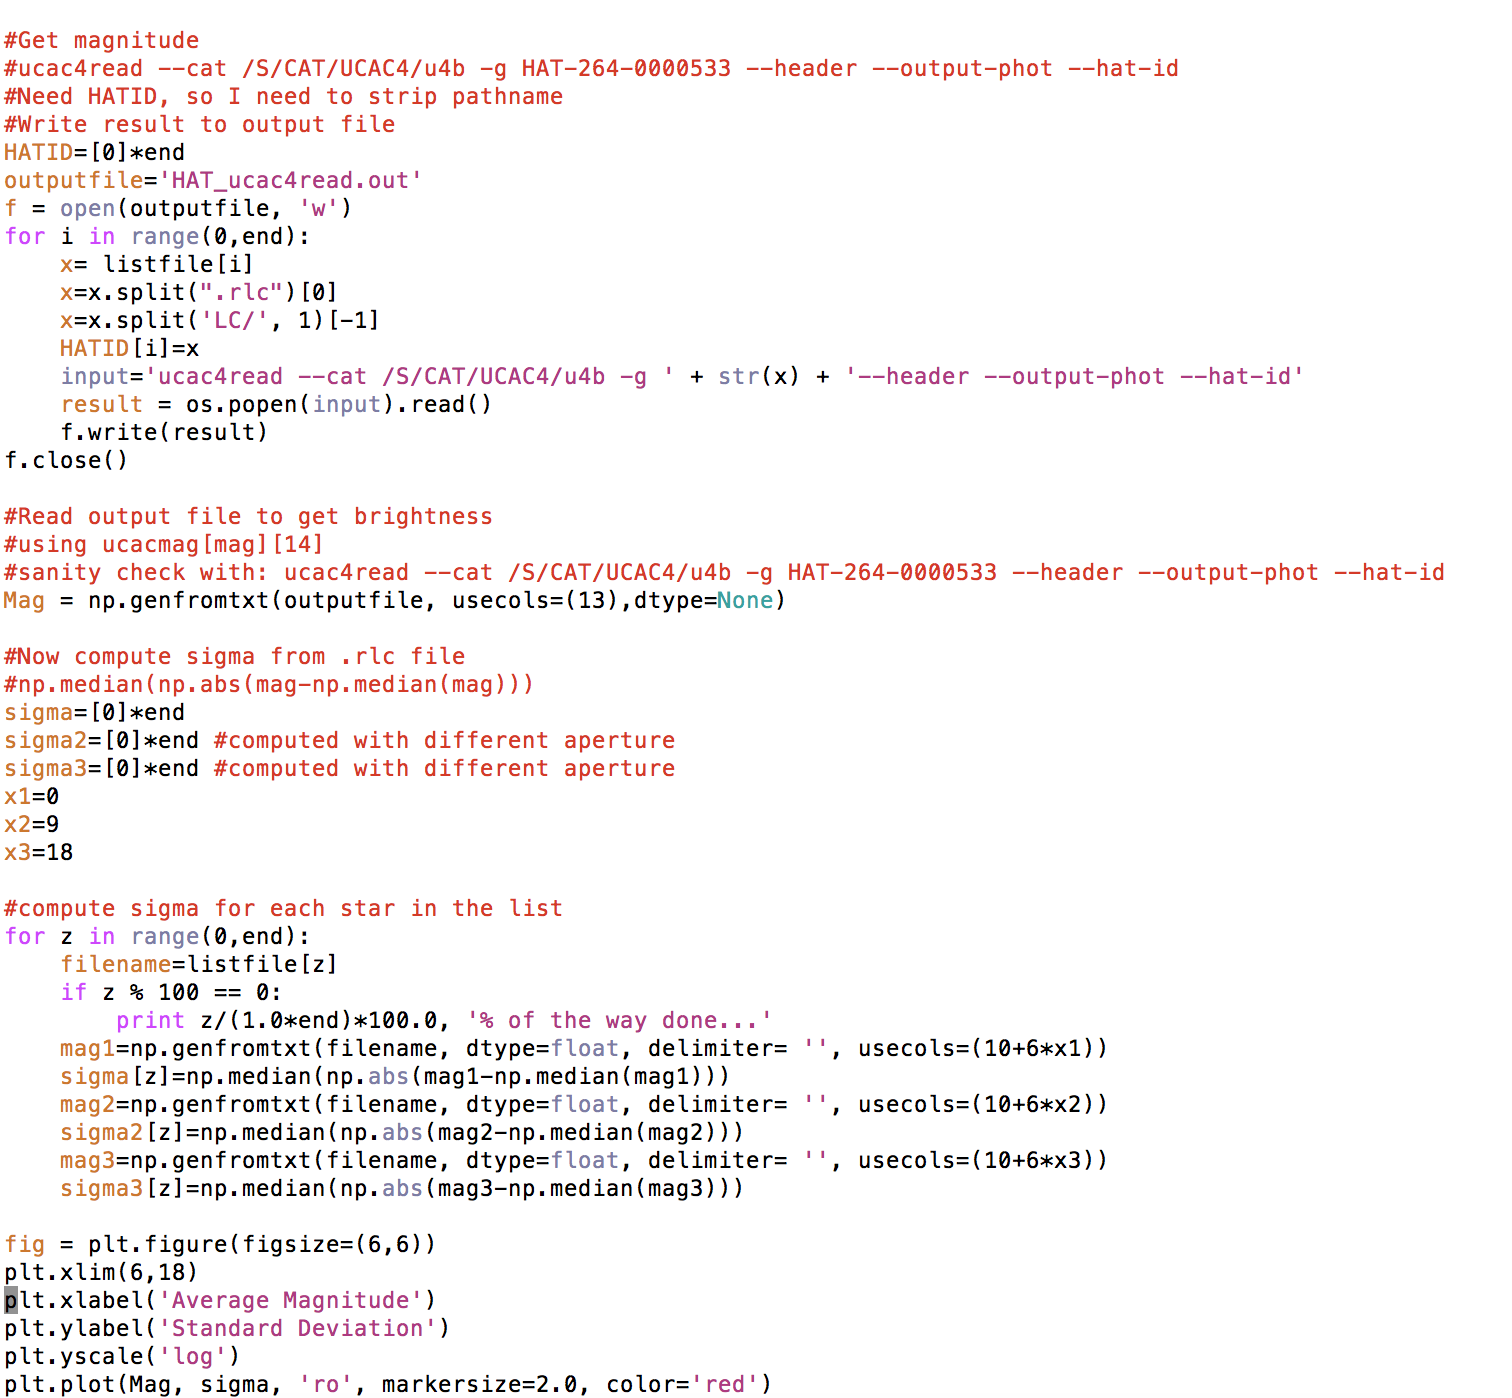
\includegraphics[width=\textwidth]{StndVMag.png}\\ 
\end{center}
To look up information on a particular star, use the \textbf{ucac4read} command, which will output the following information: HAT ID, RA, DEC, Object Type, whether or not it's a double star, magnitude, sigma of the mag, etc. 
The plots generated are shown below.
\begin{center}
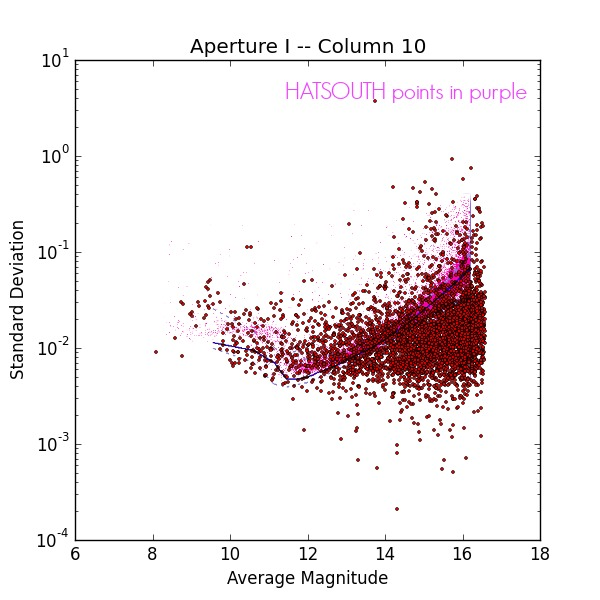
\includegraphics[width=0.8\textwidth]{Mag_Sigma1_comp.jpg}\\ 
\end{center}
\begin{center}
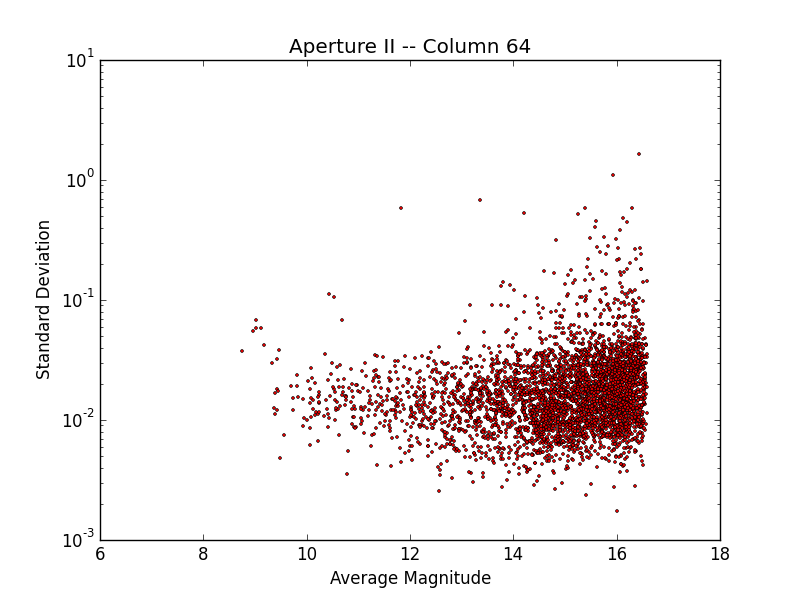
\includegraphics[width=0.8\textwidth]{Mag_Sigma2.png}\\ 
\end{center}
\begin{center}
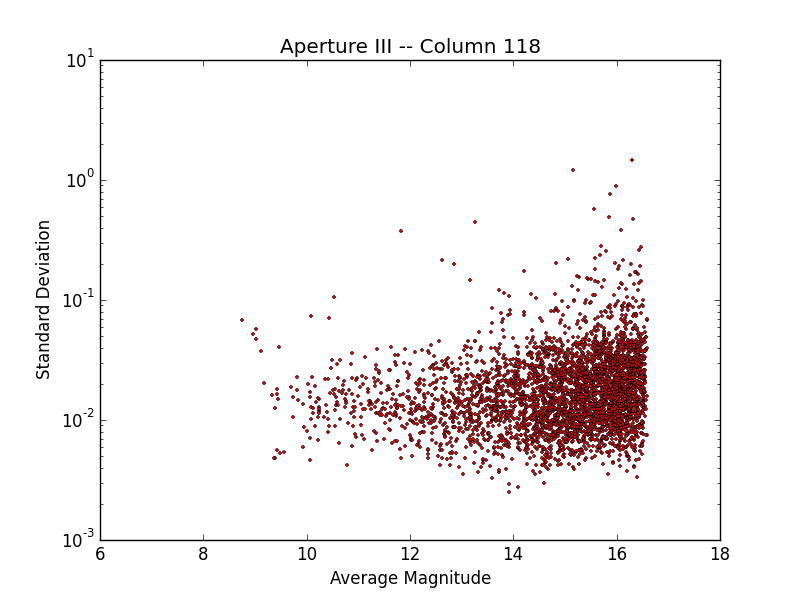
\includegraphics[width=0.8\textwidth]{Mag_Sigma3.png}\\ 
\end{center}
The three separate plots separated by a distinct aperture selection used to compute the standard deviation (np.median(np.abs(mag-np.median(mag))). Plots include all of the sources in the sub-frame. 
Unlike the example from the HATSouth survey, the overall structure is much more scattered about a more modestly increasing standard deviation for saturated stars. The standard deviation is lower for dimmer stars as compared to HATSOUTH, which you can see from the comparison plot (Mag\_Sigma1\_comp.jpg) where I have overplotted the HATSOUTH points you sent me as a reference. 
Chelsea says this difference in the scatter plots is due to blending. For many of the faint stars, we have counted lights leaking from neighboring bright stars, which make the photon noise smaller than it should be. 
\textcolor{purple}{\textit{Now I just need to do many group of experiments and have a set of these plots and pick the best. 
Chelsea says that the subtraction kernel setting is far from optimal. For raw light curves, we should be able to push down by an order of magnitude.}}

\pagebreak

\section*{Second Light Curve Batch Results: \hl{\textbf{b}/0, \textbf{i}/0, and \textbf{d}=1/1}}
\textbf{Changes made:} \\
I first made changes to the high resolution photometry with subtracted images. More specifically, I am adjust the tuning parameters: \textbf{b}, \textbf{i}, and \textbf{d}, which are set the script \textbf{melinda\_run\_ficonv.py}.
The first batch of light curves contained parameters: \textbf{b}/2, \textbf{i}/3, and \textbf{d}=3/3 \\
\textit{Remember \textbf{b} is the polynomial order fit to the background, so this was a second-order polynomial (likely too high), \textbf{i} was the order of the polynomial fit to the flux of the light curve, here a third-order polynomial (also likely too high), and \textbf{d=x/y} which is a ratio of the  half-size of the discrete kernel to the polynomial order \textbf{y} (again, probably too high).}\\
This second batch of light curves contains parameters: \textbf{b}/0, \textbf{i}/0, and \textbf{d}=1/1 \\
\textit{Files are simply overwritten and therefore I do not need to remove prior files.}\\
The \textbf{fiarith} command line subtraction is automated and already included in \textbf{melinda\_run\_ficonv.py}, so this process is completely streamlined. Next, I run the high-resolution photometry script \textbf{melinda\_run\_iphot.py}. This is followed by collecting the light curves with the bash script \textbf{melinda\_lc\_gen.sh}. This file takes a bit to run (also around 30 minutes or so). 
This will generate the light curves, which are located here: \textbf{/nfs/phs11/ar0/S/PROJ/msoares/201509\_K20\_ISM\_OpenClusters/IMSUB/LC}. \\
Again, I download all the data for this second batch.\\

\section*{Folding Light Curves}
I do not need to worry about folding light curves yet, as I still should focus on optimizing ims parameters. In the future, however, I will be folding candidate light curves.

\textcolor{purple}{\textbf{Next Mission: Generate Rotation Curve By End of November!}}\\ 
I do  not need to have the best precision to generate the rotation curve. The worst case will be just present the measurement for a few specific known targets. \textit{We might have enough time to reproduce the period .vs. B-V figure from the reference Chelsea sent me.} An example of such a plot from the Nardiello et al. 2014 paper is shown below. \\
\begin{center}
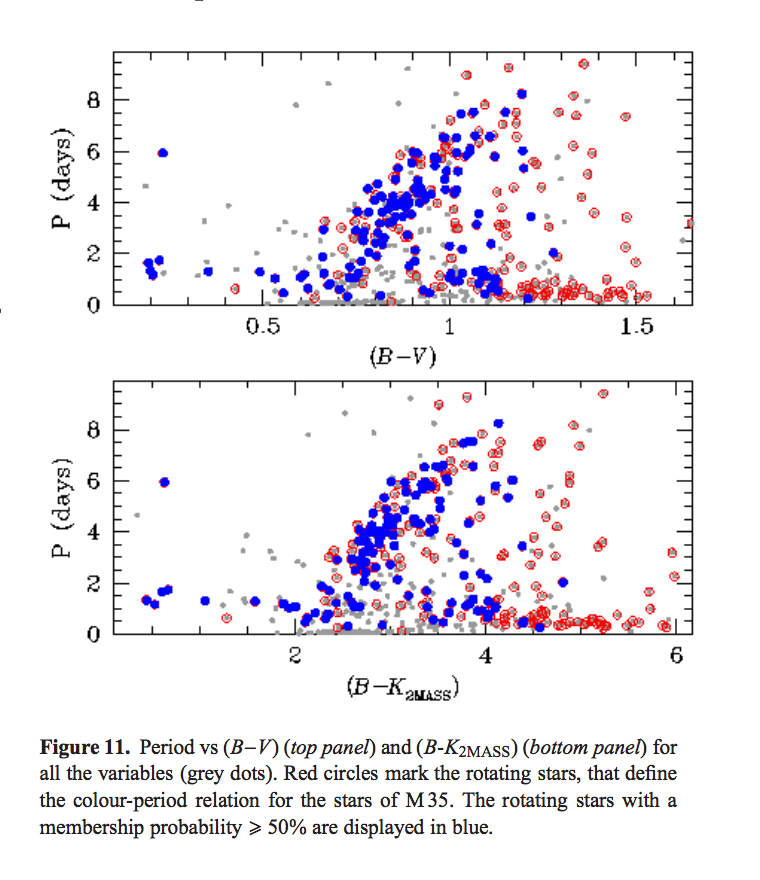
\includegraphics[width=0.4\textwidth]{reproduce2.png}
\end{center}